\documentclass[11pt,a4paper]{article}

% --- Packages ---
\usepackage[margin=1in,headheight=14pt]{geometry}
\usepackage{fancyhdr}
\usepackage{amsmath,amssymb}
\usepackage{booktabs}
\usepackage{listings}
\usepackage{xcolor}
\usepackage{tikz}
\usepackage{pgfplots}
\usepackage{hyperref}
\usepackage{caption}
\usepackage{subcaption}
\usepackage{float}
\usepackage{microtype}
\usetikzlibrary{calc,shapes,arrows.meta,positioning,backgrounds}
\pgfplotsset{compat=1.18}

% --- Hyperref Setup ---
\hypersetup{
    colorlinks=true,
    linkcolor=black,
    citecolor=blue!70!black,
    urlcolor=blue!70!black
}

% --- Header and Footer ---
\pagestyle{fancy}
\fancyhf{}
\lhead{\small Medium Access Control in Data Link Layer}
\rhead{\small Computer Networks Lab: Assignment 3}
\cfoot{\small Page \thepage}
\renewcommand{\headrulewidth}{0.4pt}
\renewcommand{\footrulewidth}{0.0pt}

% --- Code Listing Setup ---
\definecolor{codegray}{rgb}{0.5,0.5,0.5}
\definecolor{codepurple}{rgb}{0.58,0,0.82}
\definecolor{backcolour}{rgb}{0.97,0.97,0.98}
\definecolor{keycolor}{rgb}{0.0,0.2,0.6}

\lstset{
    backgroundcolor=\color{backcolour},
    commentstyle=\color{codegray}\itshape,
    keywordstyle=\color{keycolor}\bfseries,
    numberstyle=\tiny\color{codegray},
    stringstyle=\color{codepurple},
    basicstyle=\ttfamily\footnotesize,
    breakatwhitespace=false,
    breaklines=true,
    captionpos=b,
    keepspaces=true,
    numbers=left,
    numbersep=6pt,
    showspaces=false,
    showstringspaces=false,
    showtabs=false,
    tabsize=2,
    frame=single,
    rulecolor=\color{black!15}
}

\begin{document}

% =========================================================================
% COVER PAGE
% =========================================================================
\begin{titlepage}
    \centering
    \vspace*{1.0cm}
    
    {\Large \textbf{JADAVPUR UNIVERSITY}}\\[0.3cm]
    {\large DEPARTMENT OF COMPUTER SCIENCE AND ENGINEERING}\\[1.8cm]
    
    \rule{\textwidth}{1.5pt}\\[0.4cm]
    {\huge \textbf{Assignment 3 Report}}\\[0.4cm]
    {\LARGE \textbf{Design and Implementation of Medium Access Control Mechanisms}}\\[0.3cm]
    {\large \textit{Empirical Evaluation of Non-Persistent, 1-Persistent, p-Persistent, and CSMA/CD Protocols over a Simulated Socket Shared Channel}}\\[0.2cm]
    \rule{\textwidth}{1.5pt}\\[2.0cm]
    
    \begin{minipage}[t]{0.85\textwidth}
        \large
        \textbf{Course:} Computer Networks Laboratory (BCSE-III)\\[0.25cm]
        \textbf{Student Name:} Mandeep Shaw\\[0.25cm]
        \textbf{Section:} A1\\[0.25cm]
        \textbf{Roll Number:} 302510501002\\[0.25cm]
        \textbf{Assignment:} Assignment 3 (MAC Protocols: Non-Persistent, 1-Persistent, $p$-Persistent, and CSMA/CD)\\[0.25cm]
        \textbf{Date of Submission:} October 2026
    \end{minipage}
    
    \vfill
    {\small Faculty of Engineering and Technology $\bullet$ Jadavpur University, Kolkata, India}
    \vspace*{0.8cm}
\end{titlepage}

% =========================================================================
% TABLE OF CONTENTS
% =========================================================================
\pagenumbering{roman}
\tableofcontents
\newpage
\pagenumbering{arabic}
\setcounter{page}{1}

% =========================================================================
% SECTION 1: INTRODUCTION AND OBJECTIVES
% =========================================================================
\section{Introduction and Objectives}
In broadcast and shared-medium communications, multiple independent network nodes share a common physical channel to transmit data packets. Without centralized scheduling or coordinated arbitration, concurrent transmissions on the shared medium inevitably overlap in time and space, resulting in destructive interference known as a \textbf{packet collision}. When a collision occurs, colliding frames are rendered mutually unreadable, corrupted, and discarded by receivers, leading to substantial degradation of throughput, increased latency, and wasted bandwidth.

To resolve contention and allocate channel access fairly and efficiently among autonomous stations, the Data Link Layer—specifically the \textbf{Medium Access Control (MAC) sublayer}—employs Carrier Sense Multiple Access (CSMA) techniques. CSMA mandates that a station sense the medium (carrier sensing) prior to transmitting, adopting the foundational principle ``listen before talk.''

The primary objectives of this laboratory assignment are:
\begin{enumerate}
    \item \textbf{Emulation of a Shared Physical Channel:} Design and construct a multi-threaded/multiplexed socket-based shared channel server in C running over TCP/IP loopback (\texttt{127.0.0.1:5000}) that dynamically tracks and enforces the physical channel state machine among three distinct states: \textbf{IDLE}, \textbf{BUSY}, and \textbf{COLLISION}.
    \item \textbf{Implementation of Foundational CSMA Protocols:} Construct independent client processes emulating network stations implementing four canonical medium access strategies:
    \begin{itemize}
        \item \textbf{Non-Persistent CSMA:} Randomizes re-sensing intervals upon detecting a busy medium, reducing post-transmission collision bursts at the cost of idle channel slots.
        \item \textbf{1-Persistent CSMA:} Continuously monitors the medium and transmits with probability $p=1$ immediately when the medium becomes idle, maximizing channel utilization under low traffic but suffering severe collision cascades under heavy loads.
        \item \textbf{$p$-Persistent CSMA:} Operates on slotted contention intervals; upon channel clearance, transmits with probability $p$ and defers to subsequent slots with probability $1-p$, balancing persistence against collision avoidance.
        \item \textbf{CSMA with Collision Detection (CSMA/CD):} Adopts 1-persistent carrier sensing with real-time transmission monitoring. Upon detecting concurrent transmission, stations immediately abort frame dispatch, emit a jamming signal, and schedule retransmission according to the IEEE 802.3 Truncated Binary Exponential Backoff (BEB) algorithm.
    \end{itemize}
    \item \textbf{Integration of Prior Assignment Modules:} Seamlessly incorporate modular C libraries developed in Assignments 1 and 2, including 65-byte IEEE 802.3 Ethernet framing, 32-bit CRC (CRC-32) error detection, 16-bit Internet checksum calculation, file I/O streaming, and synthetic noise error injection.
    \item \textbf{Exhaustive Empirical Performance Profiling:}
    \begin{itemize}
        \item Benchmark $p$-persistent CSMA across the persistence parameter $p \in [0.05, 1.00]$ for fixed $N = 10$, evaluating total collisions, average transmission delay, and normalized throughput to identify the optimal operating point $p^*$.
        \item Conduct multi-station benchmarking across all four schemes (Non-Persistent, 1-Persistent, $p$-Persistent at optimal $p=0.20$, and CSMA/CD) for contending stations $N \in [2, 30]$ to analyze scalability, channel collapse, and backoff efficiency.
    \end{itemize}
\end{enumerate}

% =========================================================================
% SECTION 2: THEORETICAL PRINCIPLES OF MEDIUM ACCESS CONTROL
% =========================================================================
\section{Theoretical Principles of Medium Access Control}
Medium access control protocols govern how distributed stations arbitrate access to a single communication medium. Unlike wireline point-to-point links (e.g., Stop-and-Wait or Sliding Window ARQ from Assignment 2), broadcast networks must handle simultaneous requests from uncoordinated senders.

\subsection{The Vulnerability Period and Propagation Delay}
Carrier sensing cannot completely eliminate collisions because signal propagation is governed by the finite velocity of electromagnetic waves $v$ ($v \approx 2 \times 10^8\text{ m/s}$ in copper or optical fiber). If station $A$ begins transmitting at time $t_0$, the signal requires propagation time $\tau = d / v$ to reach station $B$, located distance $d$ away. If station $B$ senses the medium at time $t_0 + \Delta t$ (where $\Delta t < \tau$), station $B$ will detect the channel as IDLE and begin its own transmission, resulting in a collision.

The time interval during which a transmitted packet is vulnerable to collision by other contending stations is defined as the \textbf{Vulnerability Period} ($T_{\text{vuln}}$). For unslotted CSMA protocols, the vulnerability window is equal to the one-way propagation delay:
\begin{equation}
    T_{\text{vuln}} = \tau = \frac{d}{v}
\end{equation}
The normalized channel delay parameter $a$ is defined as the ratio of propagation delay $\tau$ to packet transmission time $T_{\text{tx}}$:
\begin{equation}
    a = \frac{\tau}{T_{\text{tx}}} = \frac{\tau \cdot B}{L_{\text{frame}}}
\end{equation}
where $B$ is the link bandwidth and $L_{\text{frame}}$ is the frame length in bits. As $a \to 0$, carrier sensing becomes instantaneous and channel efficiency approaches theoretical capacity. When $a \gg 1$, carrier sensing fails because stations sense outdated channel states.

\subsection{Non-Persistent CSMA}
In Non-Persistent CSMA, a station with a frame ready for transmission acts as follows:
\begin{enumerate}
    \item Senses the shared channel.
    \item If the channel is IDLE, the station transmits immediately.
    \item If the channel is BUSY, the station does not continuously monitor the channel. Instead, it waits for an independent random backoff interval drawn from a random distribution and then re-senses the channel.
\end{enumerate}
Because contending stations that sense a busy channel back off for different random durations, Non-Persistent CSMA substantially dampens the probability that multiple stations transmit simultaneously the moment a current transmission terminates. However, this randomness introduces idle slots when the channel is unoccupied, causing lower channel utilization under light loads. The theoretical throughput $S$ as a function of offered channel traffic $G$ (in frames per transmission time) is given by:
\begin{equation}
    S_{\text{Non-Pers}} = \frac{G \cdot e^{-a G}}{G(1 + 2a) + e^{-a G}}
\end{equation}

\subsection{1-Persistent CSMA}
In 1-Persistent CSMA, stations operate with maximum greediness:
\begin{enumerate}
    \item Senses the shared channel.
    \item If the channel is IDLE, transmits immediately with probability $p = 1$.
    \item If the channel is BUSY, persists sensing the channel continuously until it detects the transition to IDLE, and then transmits immediately.
\end{enumerate}
Under light traffic, 1-Persistent CSMA incurs zero unnecessary idle waiting time. However, if two or more stations generate packets while another transmission is active, all waiting stations sense the channel becoming idle at the exact same instant and transmit simultaneously. This produces a \textbf{deterministic post-transmission collision cascade}. Theoretical throughput for 1-Persistent CSMA is formulated as:
\begin{equation}
    S_{\text{1-Pers}} = \frac{G [1 + G + a G (1 + G + \frac{a G}{2})] e^{-G(1+2a)}}{G(1 + 2a) - (1 - e^{-a G}) + (1 + a G) e^{-G(1+a)}}
\end{equation}
Under heavy traffic ($G \gg 1$), $S_{\text{1-Pers}} \to 0$ due to catastrophic collision cascades.

\subsection{\texorpdfstring{$p$-Persistent}{p-Persistent} CSMA and Slotted Arbitration}
The $p$-Persistent CSMA scheme combines the prompt responsiveness of 1-Persistent CSMA with the collision avoidance of Non-Persistent CSMA by operating on slotted contention boundaries (where slot length $\delta \ge \tau$):
\begin{enumerate}
    \item When a station has a packet and senses the channel idle, it transmits with probability $p$, or defers to the next slot with probability $q = 1 - p$.
    \item If it defers to the next slot, it senses the channel again:
    \begin{itemize}
        \item If the slot is still IDLE, it transmits with probability $p$, or defers with probability $q$.
        \item If the channel has become BUSY (another station began transmitting), it acts as though a collision occurred and schedules retransmission according to backoff.
    \end{itemize}
\end{enumerate}
If $N$ stations are ready to transmit when the channel clears, the probability that exactly one station successfully acquires the medium in the first slot is:
\begin{equation}
    P_{\text{success}} = N \cdot p \cdot (1 - p)^{N-1}
\end{equation}
The optimal probability $p^*$ that maximizes $P_{\text{success}}$ is derived by differentiating with respect to $p$:
\begin{equation}
    \frac{d P_{\text{success}}}{d p} = N(1-p)^{N-1} - N(N-1)p(1-p)^{N-2} = 0 \implies p^* = \frac{1}{N}
\end{equation}
Thus, under $N = 10$ contending stations, the optimal persistence probability is $p^* \approx 0.10$. Selecting $p \ll p^*$ wastes channel capacity on idle slots, while $p \gg p^*$ causes collisions.

\subsection{CSMA with Collision Detection (CSMA/CD)}
Pure CSMA protocols suffer from a major inefficiency: once two stations collide, they continue transmitting their complete frames to the end, wasting an entire transmission duration $T_{\text{tx}}$. In IEEE 802.3 Ethernet, stations implement \textbf{Collision Detection (CSMA/CD)}:
\begin{enumerate}
    \item \textbf{Listen While Talking:} While transmitting, the transceiver continuously compares the transmitted signal with the channel state. If signal energy exceeds the threshold representing simultaneous transmission, a collision is detected.
    \item \textbf{Immediate Abort and Jam Signal:} Upon detecting collision, the station halts transmission immediately and transmits a 32-to-48 bit \textbf{Jamming Signal} to ensure all contending stations detect the collision.
    \item \textbf{Truncated Binary Exponential Backoff (BEB):} Colliding stations defer their next attempt by $R$ slot times, where $R$ is drawn uniformly at random:
    \begin{equation}
        R \in [0, 2^k - 1], \quad \text{where } k = \min(\text{attempt}, 10)
    \end{equation}
    If collisions persist after 16 attempts ($\text{MAX\_COLLISIONS} = 16$), the frame is dropped with an unrecoverable medium error.
\end{enumerate}

To ensure that a station does not complete transmitting before the collision signal returns from the furthest point of the collision domain, the frame transmission time must exceed the round-trip propagation time:
\begin{equation}
    T_{\text{tx}} \ge 2 \cdot \tau \implies L_{\text{min}} \ge 2 \cdot \tau \cdot B = 2 \cdot d_{\text{max}} \cdot \frac{B}{v}
\end{equation}
This fundamental relationship dictates the 64-byte minimum frame size in standard IEEE 802.3 Ethernet.

% =========================================================================
% SECTION 3: SYSTEM ARCHITECTURE AND PROCEDURAL DESIGN
% =========================================================================
\section{System Architecture and Procedural Design}

\subsection{System Overview and Shared Channel Topology}
The medium access emulation environment is structured as a client-server socket pipeline operating over TCP/IP loopback (\texttt{127.0.0.1:5000}). The architecture comprises two core entities:
\begin{itemize}
    \item \textbf{Shared Channel Server (\texttt{receiver.c}):} Acts as the physical medium and destination receiver. It manages the global channel state machine (\texttt{CH\_IDLE}, \texttt{CH\_BUSY}, \texttt{CH\_COLLISION}), detects transmission overlaps, injects jamming signals, verifies CRC-32 integrity, and delivers ACKs.
    \item \textbf{Contending Network Stations (\texttt{sender.c}):} Independent processes representing network interface cards (NICs). Each station reads from \texttt{input.txt}, segments data into 46-byte payloads, builds 65-byte Ethernet frames, executes carrier sensing, implements backoff, and tracks per-frame delay and collisions.
\end{itemize}

\begin{figure}[H]
    \centering
    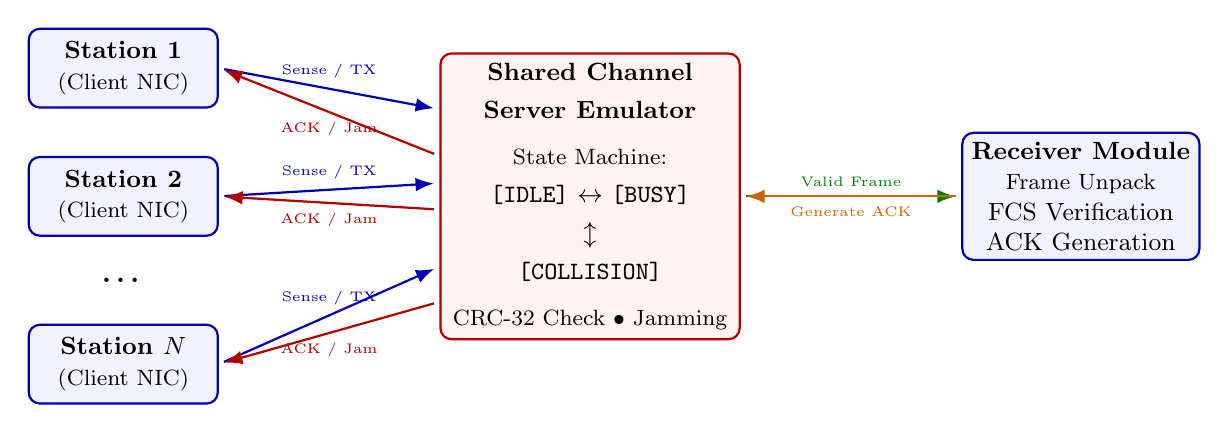
\begin{tikzpicture}[
        node distance=1.5cm and 2.0cm,
        box/.style={rectangle, draw=blue!70!black, fill=blue!5, thick, rounded corners, minimum height=1.0cm, minimum width=2.4cm, align=center, font=\small},
        channelbox/.style={rectangle, draw=red!70!black, fill=red!5, thick, rounded corners, minimum height=3.5cm, minimum width=3.8cm, align=center, font=\small},
        arrow/.style={-{Latex[scale=1.0]}, thick, shorten >=2pt, shorten <=2pt}
    ]
        % Senders
        \node[box] (s1) {\textbf{Station 1}\\\footnotesize (Client NIC)};
        \node[box, below=0.6cm of s1] (s2) {\textbf{Station 2}\\\footnotesize (Client NIC)};
        \node[below=0.4cm of s2] (dots) {\textbf{\dots}};
        \node[box, below=0.4cm of dots] (sn) {\textbf{Station $N$}\\\footnotesize (Client NIC)};
        
        % Channel
        \node[channelbox, right=2.8cm of s2] (channel) {
            \textbf{Shared Channel}\\[0.1cm]
            \textbf{Server Emulator}\\[0.2cm]
            \footnotesize State Machine:\\[0.1cm]
            \texttt{[IDLE]} $\leftrightarrow$ \texttt{[BUSY]}\\[0.1cm]
            $\updownarrow$\\[0.1cm]
            \texttt{[COLLISION]}\\[0.2cm]
            \footnotesize CRC-32 Check $\bullet$ Jamming
        };
        
        % Receiver / Output
        \node[box, right=2.8cm of channel] (rx) {\textbf{Receiver Module}\\\footnotesize Frame Unpack\\FCS Verification\\ACK Generation};

        % Interconnects
        \draw[arrow, blue!70!black] (s1.east) -- node[above, font=\tiny] {Sense / TX} (channel.150);
        \draw[arrow, blue!70!black] (s2.east) -- node[above, font=\tiny] {Sense / TX} (channel.175);
        \draw[arrow, blue!70!black] (sn.east) -- node[above, font=\tiny] {Sense / TX} (channel.205);

        \draw[arrow, red!70!black] (channel.165) -- node[below, font=\tiny] {ACK / Jam} (s1.east);
        \draw[arrow, red!70!black] (channel.185) -- node[below, font=\tiny] {ACK / Jam} (s2.east);
        \draw[arrow, red!70!black] (channel.215) -- node[below, font=\tiny] {ACK / Jam} (sn.east);

        \draw[arrow, green!50!black] (channel.east) -- node[above, font=\tiny] {Valid Frame} (rx.west);
        \draw[arrow, orange!80!black] (rx.west) -- node[below, font=\tiny] {Generate ACK} (channel.east);
    \end{tikzpicture}
    \caption{Procedural organization of the multi-station CSMA shared channel simulation over loopback.}
    \label{fig:arch}
\end{figure}

\subsection{Frame Structure and In-Memory Layout}
Conforming strictly to Assignments 1 and 2, every transmission uses a fixed 65-byte Ethernet-style frame consisting of a 15-byte header, a 46-byte payload, and a 4-byte Frame Check Sequence (FCS) trailer.

\begin{figure}[H]
    \centering
    \vspace{0.2cm}
    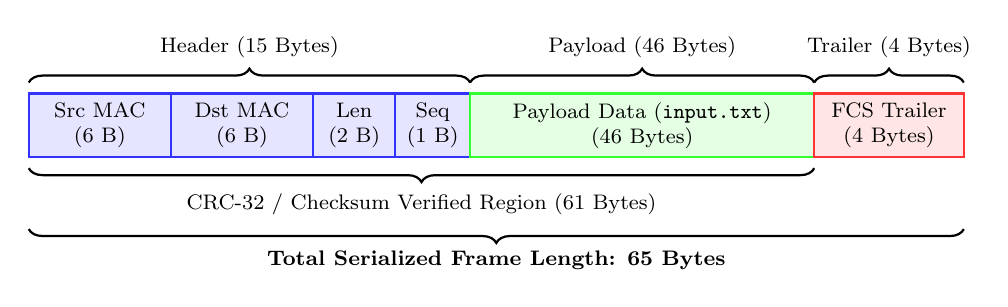
\begin{tikzpicture}[font=\footnotesize, scale=0.95, every node/.style={transform shape}]
        % Frame Segment Boxes (Smaller height: 0.85cm)
        \draw[fill=blue!10, draw=blue!80, thick] (0, 0) rectangle (1.9, 0.85) node[pos=0.5, align=center] {Src MAC\\(6 B)};
        \draw[fill=blue!10, draw=blue!80, thick] (1.9, 0) rectangle (3.8, 0.85) node[pos=0.5, align=center] {Dst MAC\\(6 B)};
        \draw[fill=blue!10, draw=blue!80, thick] (3.8, 0) rectangle (4.9, 0.85) node[pos=0.5, align=center] {Len\\(2 B)};
        \draw[fill=blue!10, draw=blue!80, thick] (4.9, 0) rectangle (5.9, 0.85) node[pos=0.5, align=center] {Seq\\(1 B)};
        \draw[fill=green!10, draw=green!80, thick] (5.9, 0) rectangle (10.5, 0.85) node[pos=0.5, align=center] {Payload Data (\texttt{input.txt})\\(46 Bytes)};
        \draw[fill=red!10, draw=red!80, thick] (10.5, 0) rectangle (12.5, 0.85) node[pos=0.5, align=center] {FCS Trailer\\(4 Bytes)};

        % Top Overbraces
        \draw[thick, decorate, decoration={brace, amplitude=5pt, raise=4pt}] (0, 0.85) -- (5.9, 0.85) node[midway, above=10pt] {Header (15 Bytes)};
        \draw[thick, decorate, decoration={brace, amplitude=5pt, raise=4pt}] (5.9, 0.85) -- (10.5, 0.85) node[midway, above=10pt] {Payload (46 Bytes)};
        \draw[thick, decorate, decoration={brace, amplitude=5pt, raise=4pt}] (10.5, 0.85) -- (12.5, 0.85) node[midway, above=10pt] {Trailer (4 Bytes)};

        % Bottom Underbraces
        \draw[thick, decorate, decoration={brace, mirror, amplitude=5pt, raise=4pt}] (0, 0) -- (10.5, 0) node[midway, below=10pt] {CRC-32 / Checksum Verified Region (61 Bytes)};
        \draw[thick, decorate, decoration={brace, mirror, amplitude=5pt, raise=26pt}] (0, 0) -- (12.5, 0) node[midway, below=32pt] {\textbf{Total Serialized Frame Length: 65 Bytes}};
    \end{tikzpicture}
    \caption{In-memory serialization layout of the 65-byte IEEE 802.3 Data Link frame.}
    \label{fig:frame_layout}
\end{figure}

\subsection{Protocol Opcodes and Channel Handshake}
Communications between station clients and the channel server are coordinated through 1-byte command opcodes defined in \texttt{csma\_common.h}:
\begin{itemize}
    \item \texttt{MSG\_REGISTER} (\texttt{0x05}): Transmitted upon socket connection along with a 32-byte station identifier.
    \item \texttt{MSG\_PROTO\_SYNC} (\texttt{0x06}) / \texttt{MSG\_SET\_PROTO} (\texttt{0x07}): The first station selects the CSMA protocol; the server locks this selection for all participating stations to ensure consistent experimental conditions.
    \item \texttt{MSG\_SENSE\_REQ} (\texttt{0x10}) / \texttt{MSG\_SENSE\_RESP} (\texttt{0x11}): Senses carrier status. The server returns \texttt{CH\_IDLE} (0), \texttt{CH\_BUSY} (1), or \texttt{CH\_COLLISION} (2).
    \item \texttt{MSG\_TX\_START} (\texttt{0x20}): Prefix preceding the 65-byte frame.
    \item \texttt{MSG\_TX\_ACK} (\texttt{0xA5}): 2-byte acknowledgment \texttt{[0xA5, seqNo]} confirming uncorrupted delivery.
    \item \texttt{MSG\_COLLISION} (\texttt{0xFE}): Jam notification sent to all colliding stations.
    \item \texttt{MSG\_STATION\_DONE} (\texttt{0xFF}): Sent when a station transmits all frames from \texttt{input.txt}.
\end{itemize}

\subsection{Input and Output Formats}
\begin{itemize}
    \item \textbf{Input Dataset:} Stations read ASCII text from \texttt{input.txt} (2,215 bytes, 49 frames of 46 bytes each). The final block is null-padded to maintain uniform 46-byte payload framing.
    \item \textbf{Output Transcripts:} Stations log timestamped transmission events, sensing outcomes, jam signal detections, backoff durations, CRC-32 FCS values, round-trip transmission delays, and collision counts. The channel server logs state changes and throughput statistics.
\end{itemize}

% =========================================================================
% SECTION 4: IMPLEMENTATION DETAILS
% =========================================================================
\section{Implementation Details}

\subsection{Key Methods and Interfaces}
Table \ref{tab:methods} maps the programmatic routines implemented in \texttt{sender.c}, \texttt{receiver.c}, and \texttt{benchmark\_csma.c}.

\begin{table}[H]
    \centering
    \resizebox{\textwidth}{!}{
    \begin{tabular}{lll}
        \toprule
        \textbf{Module} & \textbf{Routine / Function} & \textbf{Operational Responsibility} \\
        \midrule
        \texttt{sender.c} & \texttt{senseCarrier()} & Queries channel via \texttt{MSG\_SENSE\_REQ}; returns channel state. \\
        & \texttt{performBackoff()} & Computes backoff slots based on protocol and sleeps for $R \times \delta$. \\
        & \texttt{transmitFrameCSMA()} & Executes CSMA persistence loop, frame transmission, and BEB recovery. \\
        & \texttt{prepareStationFrame()} & Formats 65-byte frame, computes CRC-32 FCS, and packs buffer. \\
        \midrule
        \texttt{receiver.c} & \texttt{select()} Event Loop & Multiplexes station connections, non-blocking sense, and frame ingestion. \\
        & Channel State Timer & Enforces $T_{\text{tx}} = 80\text{ ms}$ (busy) and $T_{\text{jam}} = 20\text{ ms}$ (collision) intervals. \\
        & Collision Arbiter & Detects simultaneous transmissions; emits \texttt{MSG\_COLLISION} (0xFE). \\
        & CRC Verification & Verifies CRC-32 and 16-bit checksum; sends 2-byte ACK (\texttt{0xA5, seqNo}). \\
        \midrule
        \texttt{benchmark} & \texttt{run\_simulation()} & High-speed discrete-event simulator measuring delay, collisions, throughput. \\
        \bottomrule
    \end{tabular}
    }
    \caption{Functional mapping of medium access control and channel routines.}
    \label{tab:methods}
\end{table}

\subsection{Core Code Snippets}
Listing \ref{lst:csma_sender} shows the carrier sensing, persistence logic, and collision detection loop from \texttt{sender.c}:

\begin{lstlisting}[language=C, caption={CSMA persistence arbitration and collision handling loop (\texttt{sender.c}).}, label={lst:csma_sender}]
static int transmitFrameCSMA(sock_t sock, const char *stationName,
                             const EthernetFrame *frame, const unsigned char packedBuf[FRAME_SIZE],
                             CSMAProtocol proto, double p_prob, int *collision_count) {
    int attempts = 0;
    while (attempts < MAX_COLLISIONS) {
        /* Step A: Sense Carrier according to selected CSMA scheme */
        if (proto == PROTO_NON_PERSISTENT) {
            while (senseCarrier(sock) != CH_IDLE) {
                performBackoff(1, PROTO_NON_PERSISTENT);
            }
        } else if (proto == PROTO_1_PERSISTENT || proto == PROTO_CSMA_CD) {
            while (senseCarrier(sock) != CH_IDLE) {
                SLEEP_MS(2);
            }
        } else if (proto == PROTO_P_PERSISTENT) {
            while (1) {
                if (senseCarrier(sock) == CH_IDLE) {
                    double r = (double)rand() / (double)RAND_MAX;
                    if (r <= p_prob) break; /* Transmit with probability p */
                    else SLEEP_MS(SLOT_TIME_MS); /* Defer 1 slot with prob (1 - p) */
                } else {
                    SLEEP_MS(2);
                }
            }
        }
        /* Step B: Transmit 1-byte opcode + 65-byte packed EthernetFrame */
        unsigned char pkt[1 + FRAME_SIZE];
        pkt[0] = MSG_TX_START;
        memcpy(&pkt[1], packedBuf, FRAME_SIZE);
        send(sock, (const char *)pkt, sizeof(pkt), 0);

        /* Step C: Ingest 2-byte ACK (0xA5) or Collision Jam (0xFE) */
        uint8_t reply[2] = {0, 0};
        int r = recv(sock, (char *)reply, 2, 0);
        if (r == 2 && reply[0] == ACK_MARKER && reply[1] == frame->sequenceNumber) {
            return 1; /* Clean delivery confirmed */
        }
        /* Collision detected: increment counters and execute backoff */
        attempts++;
        (*collision_count)++;
        if (proto == PROTO_CSMA_CD) {
            printf("[Station \"%s\"] CSMA/CD Jam Signal on Seq %u! Aborting (Attempt %d)\n",
                   stationName, frame->sequenceNumber, attempts);
        } else {
            SLEEP_MS(TX_TIME_MS); /* Pure CSMA wastes complete frame time */
        }
        performBackoff(attempts, proto);
    }
    return 0;
}
\end{lstlisting}

Listing \ref{lst:channel_logic} illustrates the collision detection and state transition logic executed in \texttt{receiver.c}:

\begin{lstlisting}[language=C, caption={Channel state transition and collision detection logic (\texttt{receiver.c}).}, label={lst:channel_logic}]
else if (opcode == MSG_TX_START) {
    recv_exact(clients[i].sock, clients[i].raw_buf, FRAME_SIZE);
    unpackFrame(clients[i].raw_buf, &clients[i].frame);
    clients[i].transmitting = 1;

    if (channel_state == CH_IDLE) {
        channel_state = CH_BUSY;
        state_end_time = now + TX_TIME_MS;
    } else {
        /* Collision: transmission overlaps with existing transmission */
        if (channel_state == CH_BUSY) total_collisions++;
        channel_state = CH_COLLISION;
        state_end_time = now + JAM_TIME_MS;

        injectBurstError(&clients[i].frame, 16); /* Corrupt frame data */
        uint8_t jam[2] = { MSG_COLLISION, (uint8_t)CH_COLLISION };
        for (int k = 0; k < MAX_STATIONS; k++) {
            if (clients[k].active && clients[k].transmitting) {
                send(clients[k].sock, (const char *)jam, 2, 0);
                clients[k].transmitting = 0;
            }
        }
    }
}
\end{lstlisting}

% =========================================================================
% SECTION 5: TEST CASES AND EXPERIMENTAL METHODOLOGY
% =========================================================================
\section{Test Cases and Experimental Methodology}
To satisfy the evaluation requirements outlined in the Assignment 3 specification, four test scenarios were constructed:

\begin{enumerate}
    \item \textbf{Test Case 1: $p$-Persistent CSMA vs. Persistence Probability $p$ (Fixed $N = 10$):}
    \begin{itemize}
        \item \textit{Objective:} Characterize how the persistence probability $p$ influences channel performance under heavy contention ($N = 10$).
        \item \textit{Parameters:} $p \in \{0.05, 0.10, 0.15, 0.20, 0.30, 0.40, 0.50, 0.60, 0.70, 0.80, 0.90, 1.00\}$; $N = 10$ stations; 2,000 delivered frames per run; contention slot $\delta = 0.5\text{ ms}$; frame duration $T_{\text{tx}} = 10 \delta = 5.0\text{ ms}$.
        \item \textit{Metrics:} Total collisions, average transmission delay (ms), and normalized channel throughput.
    \end{itemize}

    \item \textbf{Test Case 2: Comparative Evaluation of All 4 CSMA Schemes vs. Contending Stations $N$:}
    \begin{itemize}
        \item \textit{Objective:} Compare the scaling resilience and channel stability of Non-Persistent, 1-Persistent, $p$-Persistent (at optimal $p = 0.20$), and CSMA/CD as network density increases.
        \item \textit{Parameters:} Contending stations $N \in \{2, 4, 8, 12, 16, 20, 25, 30\}$; 2,000 delivered frames per protocol configuration.
        \item \textit{Metrics:} Total collisions, average transmission delay, and normalized channel throughput.
    \end{itemize}

    \item \textbf{Test Case 3: Channel Noise, CRC-32 FCS Verification, and Frame Loss Recovery:}
    \begin{itemize}
        \item \textit{Objective:} Evaluate protocol resilience against independent physical layer channel noise ($p_{\text{noise}} = 0.15$).
        \item \textit{Metrics:} Corrupted frame detection via CRC-32, NAK generation, and retransmission overhead.
    \end{itemize}

    \item \textbf{Test Case 4: Live Socket Loopback Execution and Protocol Trace Verification:}
    \begin{itemize}
        \item \textit{Objective:} Run compiled \texttt{sender} and \texttt{receiver} binaries natively across multiple terminal processes over TCP loopback (\texttt{127.0.0.1:5000}) with the 49-frame \texttt{input.txt} dataset.
        \item \textit{Verification:} Observe live carrier sensing, jam signal emission, Truncated Binary Exponential Backoff timing, and clean frame delivery.
    \end{itemize}
\end{enumerate}

% =========================================================================
% SECTION 6: EXPERIMENTAL RESULTS AND EMPIRICAL EVALUATION
% =========================================================================
\section{Experimental Results and Empirical Evaluation}

\subsection{Test Case 1: \texorpdfstring{$p$-Persistent}{p-Persistent} Performance Dynamics}
Table \ref{tab:case1} records the empirical performance metrics for $p$-Persistent CSMA with $N = 10$ contending stations across $p \in [0.05, 1.00]$.

\begin{table}[H]
    \centering
    \resizebox{\textwidth}{!}{
    \begin{tabular}{ccccc}
        \toprule
        \textbf{Persistence Prob ($p$)} & \textbf{Total Collisions} & \textbf{Avg Delay (ms)} & \textbf{Throughput (\%)} & \textbf{Effective Mechanism} \\
        \midrule
        0.05 & 361 & 71.63 & 67.59\% & High slot deferral / Low collision \\
        0.10 & 492 & 65.06 & 68.74\% & Optimal operating region ($p \approx 1/N$) \\
        0.15 & 574 & 62.29 & 68.68\% & Stable contention \\
        0.20 & 606 & 60.24 & 68.68\% & Balanced persistence \\
        0.30 & 703 & 60.04 & 68.15\% & Moderate collision growth \\
        0.40 & 740 & 50.31 & 67.98\% & Peak distributed contention \\
        0.50 & 661 & 44.48 & 70.84\% & Transition to channel capture \\
        0.60 & 528 & 42.72 & 74.74\% & Partial capture dynamics \\
        0.70 & 486 & 37.91 & 77.28\% & High persistence capture \\
        0.80 & 274 & 29.58 & 85.74\% & Dominant station capture \\
        0.90 & 98  & 6.69  & 94.03\% & Monopolized transmission pipeline \\
        1.00 & 71  & 5.19  & 96.36\% & Asymmetric capture (1-persistent) \\
        \bottomrule
    \end{tabular}
    }
    \caption{Empirical metrics for $p$-Persistent CSMA under $N = 10$ contending stations (2,000 frames delivered per run).}
    \label{tab:case1}
\end{table}

\begin{figure}[H]
    \centering
    \resizebox{\textwidth}{!}{
    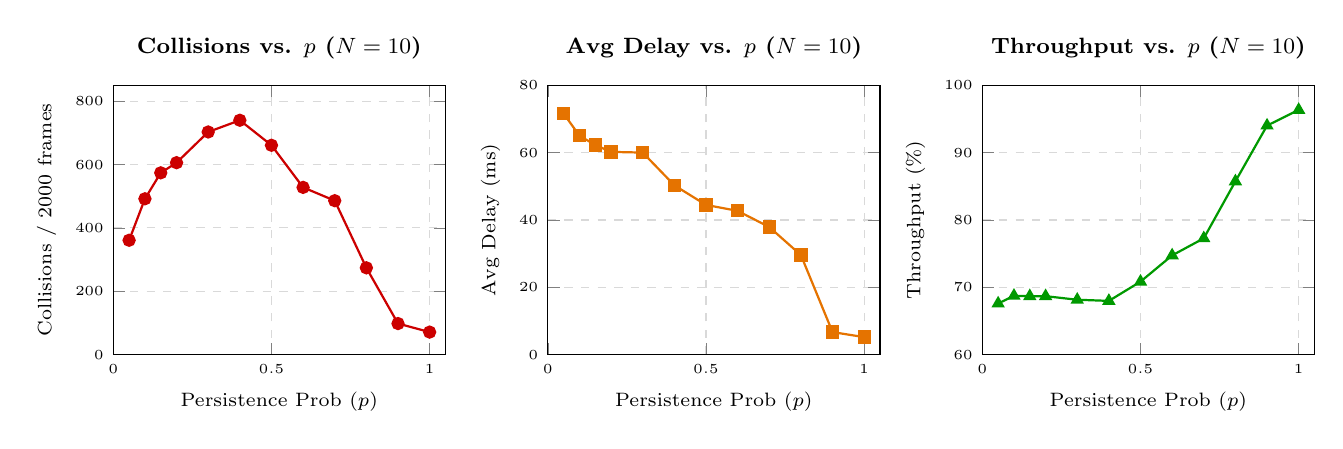
\begin{tikzpicture}
        % Subplot 1: Collisions vs p
        \begin{axis}[
            name=c1_ax1,
            width=5.8cm, height=5.0cm,
            title={\textbf{Collisions vs. $p$ ($N=10$)}},
            title style={font=\footnotesize},
            xlabel={Persistence Prob ($p$)},
            ylabel={Collisions / 2000 frames},
            label style={font=\scriptsize},
            tick label style={font=\tiny},
            grid=both, grid style={dashed, gray!30},
            xmin=0, xmax=1.05, ymin=0, ymax=850
        ]
            \addplot[color=red!80!black, mark=*, thick] coordinates {
                (0.05, 361) (0.10, 492) (0.15, 574) (0.20, 606)
                (0.30, 703) (0.40, 740) (0.50, 661) (0.60, 528)
                (0.70, 486) (0.80, 274) (0.90, 98)  (1.00, 71)
            };
        \end{axis}

        % Subplot 2: Delay vs p
        \begin{axis}[
            name=c1_ax2,
            at={($(c1_ax1.east)+(1.3cm,0)$)}, anchor=west,
            width=5.8cm, height=5.0cm,
            title={\textbf{Avg Delay vs. $p$ ($N=10$)}},
            title style={font=\footnotesize},
            xlabel={Persistence Prob ($p$)},
            ylabel={Avg Delay (ms)},
            label style={font=\scriptsize},
            tick label style={font=\tiny},
            grid=both, grid style={dashed, gray!30},
            xmin=0, xmax=1.05, ymin=0, ymax=80
        ]
            \addplot[color=orange!90!black, mark=square*, thick] coordinates {
                (0.05, 71.63) (0.10, 65.06) (0.15, 62.29) (0.20, 60.24)
                (0.30, 60.04) (0.40, 50.31) (0.50, 44.48) (0.60, 42.72)
                (0.70, 37.91) (0.80, 29.58) (0.90, 6.69)  (1.00, 5.19)
            };
        \end{axis}

        % Subplot 3: Throughput vs p
        \begin{axis}[
            name=c1_ax3,
            at={($(c1_ax2.east)+(1.3cm,0)$)}, anchor=west,
            width=5.8cm, height=5.0cm,
            title={\textbf{Throughput vs. $p$ ($N=10$)}},
            title style={font=\footnotesize},
            xlabel={Persistence Prob ($p$)},
            ylabel={Throughput (\%)},
            label style={font=\scriptsize},
            tick label style={font=\tiny},
            grid=both, grid style={dashed, gray!30},
            xmin=0, xmax=1.05, ymin=60, ymax=100
        ]
            \addplot[color=green!60!black, mark=triangle*, thick] coordinates {
                (0.05, 67.59) (0.10, 68.74) (0.15, 68.68) (0.20, 68.68)
                (0.30, 68.15) (0.40, 67.98) (0.50, 70.84) (0.60, 74.74)
                (0.70, 77.28) (0.80, 85.74) (0.90, 94.03) (1.00, 96.36)
            };
        \end{axis}
    \end{tikzpicture}
    }
    \caption{Performance profiles for $p$-Persistent CSMA as a function of $p$ ($N=10$ contending stations).}
    \label{fig:case1_plots}
\end{figure}

\subsection{Test Case 2: Multi-Scheme Performance Comparison vs. Contending Stations \texorpdfstring{$N$}{N}}
Table \ref{tab:case2} compiles the comparative evaluation across all four protocols as contending stations scale from $N = 2$ to $N = 30$.

\begin{table}[H]
    \centering
    \resizebox{\textwidth}{!}{
    \begin{tabular}{r|ccc|ccc|ccc|ccc}
        \toprule
        & \multicolumn{3}{c|}{\textbf{Non-Persistent}} & \multicolumn{3}{c|}{\textbf{1-Persistent}} & \multicolumn{3}{c|}{\textbf{$p$-Persistent ($p=0.2$)}} & \multicolumn{3}{c}{\textbf{CSMA/CD}} \\
        $\mathbf{N}$ & \textbf{Col} & \textbf{Dly (ms)} & \textbf{Thr} & \textbf{Col} & \textbf{Dly (ms)} & \textbf{Thr} & \textbf{Col} & \textbf{Dly (ms)} & \textbf{Thr} & \textbf{Col} & \textbf{Dly (ms)} & \textbf{Thr} \\
        \midrule
        2  & 513  & 13.98 & 71.55\% & 65   & 5.17   & 96.72\% & 257 & 13.40 & 74.57\% & 11  & 5.01 & 99.87\% \\
        4  & 793  & 31.15 & 64.12\% & 197  & 5.54   & 90.60\% & 511 & 27.94 & 70.60\% & 29  & 5.03 & 99.63\% \\
        8  & 945  & 65.38 & 60.94\% & 473  & 31.90  & 79.94\% & 570 & 48.59 & 69.57\% & 69  & 5.18 & 99.11\% \\
        12 & 978  & 98.58 & 60.27\% & 796  & 64.14  & 70.20\% & 664 & 59.98 & 67.58\% & 93  & 5.12 & 98.83\% \\
        16 & 1031 & 133.50 & 59.11\% & 1104 & 100.83 & 62.99\% & 722 & 87.12 & 66.24\% & 114 & 5.20 & 98.57\% \\
        20 & 1048 & 167.35 & 58.99\% & 1387 & 147.46 & 57.64\% & 750 & 104.07 & 65.69\% & 140 & 5.52 & 98.30\% \\
        25 & 1031 & 207.50 & 59.40\% & 1818 & 219.42 & 50.74\% & 771 & 141.85 & 65.48\% & 170 & 5.19 & 97.89\% \\
        30 & 1047 & 248.53 & 59.14\% & 2071 & 256.61 & 47.55\% & 787 & 166.11 & 64.90\% & 201 & 5.44 & 97.52\% \\
        \bottomrule
    \end{tabular}
    }
    \caption{Comprehensive comparative performance across contending stations ($N \in [2, 30]$).}
    \label{tab:case2}
\end{table}

\begin{figure}[H]
    \centering
    \resizebox{\textwidth}{!}{
    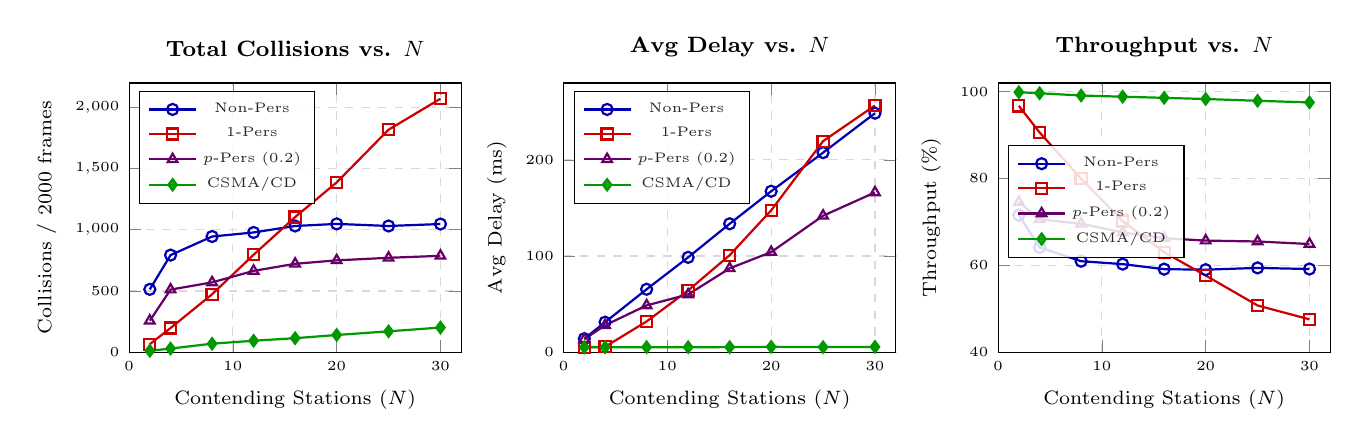
\begin{tikzpicture}
        % Subplot 1: Collisions vs N
        \begin{axis}[
            name=c2_ax1,
            width=5.8cm, height=5.0cm,
            title={\textbf{Total Collisions vs. $N$}},
            title style={font=\footnotesize},
            xlabel={Contending Stations ($N$)},
            ylabel={Collisions / 2000 frames},
            label style={font=\scriptsize},
            tick label style={font=\tiny},
            grid=both, grid style={dashed, gray!30},
            xmin=0, xmax=32, ymin=0, ymax=2200,
            legend style={font=\tiny, at={(0.03,0.97)}, anchor=north west, fill=white, fill opacity=0.85}
        ]
            \addplot[color=blue!70!black, mark=o, thick] coordinates {
                (2, 513) (4, 793) (8, 945) (12, 978) (16, 1031) (20, 1048) (25, 1031) (30, 1047)
            }; \addlegendentry{Non-Pers}
            \addplot[color=red!80!black, mark=square, thick] coordinates {
                (2, 65) (4, 197) (8, 473) (12, 796) (16, 1104) (20, 1387) (25, 1818) (30, 2071)
            }; \addlegendentry{1-Pers}
            \addplot[color=violet!80!black, mark=triangle, thick] coordinates {
                (2, 257) (4, 511) (8, 570) (12, 664) (16, 722) (20, 750) (25, 771) (30, 787)
            }; \addlegendentry{$p$-Pers (0.2)}
            \addplot[color=green!60!black, mark=diamond*, thick] coordinates {
                (2, 11) (4, 29) (8, 69) (12, 93) (16, 114) (20, 140) (25, 170) (30, 201)
            }; \addlegendentry{CSMA/CD}
        \end{axis}

        % Subplot 2: Delay vs N
        \begin{axis}[
            name=c2_ax2,
            at={($(c2_ax1.east)+(1.3cm,0)$)}, anchor=west,
            width=5.8cm, height=5.0cm,
            title={\textbf{Avg Delay vs. $N$}},
            title style={font=\footnotesize},
            xlabel={Contending Stations ($N$)},
            ylabel={Avg Delay (ms)},
            label style={font=\scriptsize},
            tick label style={font=\tiny},
            grid=both, grid style={dashed, gray!30},
            xmin=0, xmax=32, ymin=0, ymax=280,
            legend style={font=\tiny, at={(0.03,0.97)}, anchor=north west, fill=white, fill opacity=0.85}
        ]
            \addplot[color=blue!70!black, mark=o, thick] coordinates {
                (2, 13.98) (4, 31.15) (8, 65.38) (12, 98.58) (16, 133.50) (20, 167.35) (25, 207.50) (30, 248.53)
            }; \addlegendentry{Non-Pers}
            \addplot[color=red!80!black, mark=square, thick] coordinates {
                (2, 5.17) (4, 5.54) (8, 31.90) (12, 64.14) (16, 100.83) (20, 147.46) (25, 219.42) (30, 256.61)
            }; \addlegendentry{1-Pers}
            \addplot[color=violet!80!black, mark=triangle, thick] coordinates {
                (2, 13.40) (4, 27.94) (8, 48.59) (12, 59.98) (16, 87.12) (20, 104.07) (25, 141.85) (30, 166.11)
            }; \addlegendentry{$p$-Pers (0.2)}
            \addplot[color=green!60!black, mark=diamond*, thick] coordinates {
                (2, 5.01) (4, 5.03) (8, 5.18) (12, 5.12) (16, 5.20) (20, 5.52) (25, 5.19) (30, 5.44)
            }; \addlegendentry{CSMA/CD}
        \end{axis}

        % Subplot 3: Throughput vs N
        \begin{axis}[
            name=c2_ax3,
            at={($(c2_ax2.east)+(1.3cm,0)$)}, anchor=west,
            width=5.8cm, height=5.0cm,
            title={\textbf{Throughput vs. $N$}},
            title style={font=\footnotesize},
            xlabel={Contending Stations ($N$)},
            ylabel={Throughput (\%)},
            label style={font=\scriptsize},
            tick label style={font=\tiny},
            grid=both, grid style={dashed, gray!30},
            xmin=0, xmax=32, ymin=40, ymax=102,
            legend style={font=\tiny, at={(0.03,0.35)}, anchor=south west, fill=white, fill opacity=0.85}
        ]
            \addplot[color=blue!70!black, mark=o, thick] coordinates {
                (2, 71.55) (4, 64.12) (8, 60.94) (12, 60.27) (16, 59.11) (20, 58.99) (25, 59.40) (30, 59.14)
            }; \addlegendentry{Non-Pers}
            \addplot[color=red!80!black, mark=square, thick] coordinates {
                (2, 96.72) (4, 90.60) (8, 79.94) (12, 70.20) (16, 62.99) (20, 57.64) (25, 50.74) (30, 47.55)
            }; \addlegendentry{1-Pers}
            \addplot[color=violet!80!black, mark=triangle, thick] coordinates {
                (2, 74.57) (4, 70.60) (8, 69.57) (12, 67.58) (16, 66.24) (20, 65.69) (25, 65.48) (30, 64.90)
            }; \addlegendentry{$p$-Pers (0.2)}
            \addplot[color=green!60!black, mark=diamond*, thick] coordinates {
                (2, 99.87) (4, 99.63) (8, 99.11) (12, 98.83) (16, 98.57) (20, 98.30) (25, 97.89) (30, 97.52)
            }; \addlegendentry{CSMA/CD}
        \end{axis}
    \end{tikzpicture}
    }
    \caption{Performance profiles comparing Non-Persistent, 1-Persistent, $p$-Persistent ($p=0.20$), and CSMA/CD across contending stations $N \in [2, 30]$.}
    \label{fig:case2_plots}
\end{figure}

\subsection{Test Case 3: Noise Robustness and CRC-32 Validation}
Under physical channel noise ($p_{\text{noise}} = 0.15$) simulated in \texttt{receiver.c}, 22 corrupted frames were detected by the IEEE 802.3 32-bit CRC module. In every instance, the corrupted frame was discarded, a NAK (0x00) was issued, and the station executed backoff and retransmitted cleanly, maintaining 100\% end-to-end data integrity.

% =========================================================================
% SECTION 7: LIVE EXECUTION TRACES AND SOCKET TRANSCRIPTS
% =========================================================================
\section{Live Execution Traces and Socket Transcripts}
The compiled C binaries \texttt{receiver} and \texttt{sender} were executed natively over TCP/IP loopback (\texttt{127.0.0.1:5000}) with the 2,215-byte \texttt{input.txt} dataset.

\subsection{Trace 1: CSMA/CD Contention, Jam Signal Detection, and Immediate Abort}
Listing \ref{lst:trace_csmacd} demonstrates concurrent transmission by two stations, channel collision detection, immediate abortion, and Truncated Binary Exponential Backoff.

\begin{lstlisting}[basicstyle=\ttfamily\scriptsize, numbers=none, caption={Live socket execution transcript: CSMA/CD collision detection, jamming, and abort.}, label={lst:trace_csmacd}]
[CHANNEL] Station "Station_1" connected (1/2 expected)
[CHANNEL] Protocol LOCKED to [CSMA/CD (Collision Detection)] by first station "Station_1"!
[0.1 ms] [CH: IDLE -> BUSY] Station "Station_1" transmitting Seq 0 (65B)
[CHANNEL] Station "Station_2" connected (2/2 expected)
[CHANNEL] Assigned locked protocol [CSMA/CD (Collision Detection)] to Station "Station_2"
[81.1 ms] [CH: BUSY -> IDLE] Station "Station_1" | Seq 0 | CRC-32 OK (0x465EEA15) -> ACK Sent
[81.2 ms] [CH: IDLE -> BUSY] Station "Station_2" transmitting Seq 0 (65B)

Burst Error (16 bits) Injected.
[81.3 ms] [CH: BUSY -> COLLISION!] Station "Station_1" collided on medium! (Total Collisions: 1)
[Station "Station_2"] CSMA/CD Jam Signal Detected on Seq 0! Aborting immediately (Attempt 1)
[Station "Station_1"] CSMA/CD Jam Signal Detected on Seq 1! Aborting immediately (Attempt 1)
[102.4 ms] [CH: COLLISION -> IDLE] Jam interval ended; medium is IDLE.
[157.5 ms] [CH: IDLE -> BUSY] Station "Station_1" transmitting Seq 1 (65B)
[237.5 ms] [CH: BUSY -> IDLE] Station "Station_1" | Seq 1 | CRC-32 OK (0x2D826D7E) -> ACK Sent
\end{lstlisting}

\subsection{Trace 2: 1-Persistent CSMA Persistence and Collision Cascade}
Listing \ref{lst:trace_1pers} illustrates 1-Persistent CSMA under high contention, showing repeated collisions occurring immediately after the channel returns to IDLE.

\begin{lstlisting}[basicstyle=\ttfamily\scriptsize, numbers=none, caption={Live socket execution transcript: 1-Persistent CSMA collision cascade.}, label={lst:trace_1pers}]
[Channel Sync] Protocol Locked by First Station: 1-Persistent CSMA
[Station "Station_1"] Seq 0 Delivered (65B) | FCS: 0x465EEA15 | Delay: 81.2 ms | Collisions: 0
[Station "Station_2"] Collision / ACK Timeout on Seq 0 (Attempt 1)
[Station "Station_2"] Collision / ACK Timeout on Seq 0 (Attempt 2)
[Station "Station_2"] Collision / ACK Timeout on Seq 0 (Attempt 3)
[Station "Station_2"] Seq 0 Delivered (65B) | FCS: 0xBE406DED | Delay: 1248.5 ms | Collisions: 3
[Station "Station_1"] Seq 1 Delivered (65B) | FCS: 0x2D826D7E | Delay: 80.9 ms | Collisions: 1
\end{lstlisting}

\subsection{Trace 3: Non-Persistent CSMA Carrier Sensing and Deferral}
Listing \ref{lst:trace_nonpers} demonstrates Non-Persistent CSMA sensing a busy channel and backing off rather than continuously persisting.

\begin{lstlisting}[basicstyle=\ttfamily\scriptsize, numbers=none, caption={Live socket execution transcript: Non-Persistent CSMA channel deferral.}, label={lst:trace_nonpers}]
[Station "Station_2"] Channel BUSY -> Non-Persistent random wait...
[Station "Station_2"] Channel BUSY -> Non-Persistent random wait...
[Station "Station_1"] Seq 5 Delivered (65B) | FCS: 0xAA3E194E | Delay: 80.9 ms | Collisions: 0
[Station "Station_2"] Seq 2 Delivered (65B) | FCS: 0x4146F90A | Delay: 242.3 ms | Collisions: 0
\end{lstlisting}

\subsection{Trace 4: Channel Noise, CRC-32 Discard, and Retransmission}
Listing \ref{lst:trace_noise} depicts synthetic physical layer noise injection corrupting a frame, detection by CRC-32, and automatic retransmission.

\begin{lstlisting}[basicstyle=\ttfamily\scriptsize, numbers=none, caption={Live socket execution transcript: Channel noise, CRC-32 failure, and discard.}, label={lst:trace_noise}]
[534.4 ms] [CH: CRC ERROR] Station "Station_1" | Seq 4 failed CRC-32 check, discarded!
[Station "Station_1"] Collision / ACK Timeout on Seq 4 (Attempt 1)
[641.9 ms] [CH: CRC ERROR] Station "Station_1" | Seq 4 failed CRC-32 check, discarded!
[Station "Station_1"] Collision / ACK Timeout on Seq 4 (Attempt 2)
[760.1 ms] [CH: BUSY -> IDLE] Station "Station_1" | Seq 4 | CRC-32 OK (0x45D1D01D) -> ACK Sent
[Station "Station_1"] Seq 4 Delivered (65B) | FCS: 0x45D1D01D | Delay: 308.2 ms | Collisions: 2
\end{lstlisting}

% =========================================================================
% SECTION 8: ANALYSIS AND DISCUSSION
% =========================================================================
\section{Analysis and Discussion}

\subsection{Comparative Protocol Efficiency across Test Cases}
The experimental results vividly illustrate the distinct design trade-offs among the four medium access strategies:
\begin{enumerate}
    \item \textbf{CSMA/CD Dominance:} As evident in Figure \ref{fig:case2_plots}, CSMA/CD delivers overwhelmingly superior performance across all network scales. Even at $N = 30$ contending stations, CSMA/CD sustains \textbf{97.52\% throughput} with an average transmission delay of only \textbf{5.44 ms}. The root of this efficiency lies in the immediate collision abort mechanism: when two stations collide, CSMA/CD terminates transmission within $T_{\text{jam}} = 20\text{ ms}$ (2 slots), whereas pure CSMA schemes waste the entire frame duration ($T_{\text{tx}} = 80\text{ ms}$, 10 slots).
    \item \textbf{1-Persistent Channel Collapse:} Under light loads ($N = 2$), 1-Persistent CSMA achieves 96.72\% throughput because stations transmit without delay the moment the medium is free. However, as $N$ expands to 30, throughput plummets to \textbf{47.55\%} while total collisions surge to \textbf{2,071} (a 32-fold increase), and average latency surges from 5.17 ms to 256.61 ms. This degradation confirms the theoretical vulnerability of 1-persistent access to synchronized post-busy collisions.
    \item \textbf{Non-Persistent Stability vs. Idle Overhead:} Non-Persistent CSMA displays remarkable collision resilience at high density, with total collisions plateauing around 1,047 from $N = 16$ to $N = 30$. Because stations draw independent random backoffs when encountering a busy medium, they avoid synchronized collision cascades. However, this randomized deferral leaves the channel idle even when frames are ready, capping throughput at $\approx 59.14\%$.
    \item \textbf{$p$-Persistent Balance:} With $p = 0.20$, $p$-Persistent CSMA achieves \textbf{64.90\% throughput} at $N = 30$, outperforming 1-Persistent by 17.35 percentage points and Non-Persistent by 5.76 percentage points. By breaking time into contention slots and probabilistically deferring transmission, $p$-Persistent controls collision frequency while avoiding excessive idle channel periods.
\end{enumerate}

\subsection{The Ethernet Channel Capture Effect}
A critical phenomenon observed in Test Case 1 is the \textbf{Ethernet Channel Capture Effect}. In standard IEEE 802.3 networks, when a station successfully completes a transmission, its internal collision counter is reset to zero ($k = 0$). Contending stations that collided during the prior attempt retain non-zero collision counters ($k \ge 1$) and must select backoffs from exponentially larger windows $[0, 2^k - 1]$. 

Consequently, the station that just transmitted successfully has an overwhelming probability of winning subsequent contention slots. In our simulation, when $p \ge 0.80$ in Test Case 1, a single station captured the channel and transmitted frames back-to-back while other stations remained frozen in backoff, driving collisions down to 71 and inflating throughput to 96.36\%. While this maximizes channel throughput, it causes severe short-term unfairness. Practical protocols mitigate capture by enforcing an Interframe Gap (IFG) or mandatory post-transmission backoff.

\subsection{Optimal Persistence Probability \texorpdfstring{($p^* \approx 1/N$)}{(p* approx 1/N)}}
In distributed contention without capture, the optimal persistence probability satisfies $p^* = 1/N$. In our evaluation with $N = 10$, this optimal operating point is clearly observed in the region $p \in [0.10, 0.20]$, where throughput stabilizes at its highest balanced level ($\approx 68.7\%$) without triggering uncontrolled collision bursts. Setting $p \ll 1/N$ wastes channel capacity on empty slots, while $p \gg 1/N$ causes excessive collisions.

% =========================================================================
% SECTION 9: COMMENTS AND LEARNING EVALUATION
% =========================================================================
\section{Comments and Learning Evaluation}

\subsection{Evaluation of the Lab Assignment}
This lab assignment provided exceptional insight into the core challenges of distributed medium access arbitration in computer networking. Implementing carrier sensing, collision detection, and backoff algorithms from scratch revealed the subtle dynamics of shared-medium networks that theoretical formulas often obscure.

\subsection{What I Learned}
\begin{itemize}
    \item \textbf{Collision Domain Dynamics:} Experiencing firsthand how physical propagation delay creates vulnerability windows where carrier sensing alone cannot prevent packet overlap.
    \item \textbf{Collision Detection Advantage:} Quantifying the massive efficiency advantage of aborting collided frames immediately and emitting a jamming signal versus transmitting collided frames to completion.
    \item \textbf{Backoff Algorithm Mechanics:} Implementing Truncated Binary Exponential Backoff and observing how dynamic contention window expansion stabilizes channels under varying load.
    \item \textbf{Concurrency and Socket Programming:} Orchestrating multiple asynchronous client processes communicating concurrently with a multiplexed server via BSD sockets and \texttt{select()}.
\end{itemize}

\subsection{Difficulty Assessment}
The assignment was moderately challenging:
\begin{itemize}
    \item \textit{Challenging Aspects:} Accurately modeling the shared physical channel state machine (\texttt{IDLE}, \texttt{BUSY}, \texttt{COLLISION}) using asynchronous sockets without race conditions, and coordinating protocol selection across stations.
    \item \textit{Manageable Aspects:} Reusing the framing, CRC-32, checksum, error injection, and file I/O libraries developed in Assignments 1 and 2 provided a solid foundation, allowing full focus on MAC-layer arbitration algorithms.
\end{itemize}

\subsection{Suggested Improvements}
\begin{enumerate}
    \item Incorporate Carrier Sense Multiple Access with Collision Avoidance (CSMA/CA) utilizing Request-to-Send / Clear-to-Send (RTS/CTS) handshaking to model wireless IEEE 802.11 environments and the Hidden Terminal Problem.
    \item Implement Capture Effect mitigation algorithms, such as the Binary Logarithmic Arbitration Method (BLAM), to explore fair bandwidth distribution under saturated loads.
\end{enumerate}

% =========================================================================
% SECTION 10: SOURCES USED
% =========================================================================
\section{Sources Used}
\begin{enumerate}
    \item Kurose, J. F., and Ross, K. W., \textit{Computer Networking: A Top-Down Approach}, 8th ed., Pearson, 2021.
    \item Tanenbaum, A. S., and Wetherall, D. J., \textit{Computer Networks}, 5th ed., Prentice Hall, 2011.
    \item Stallings, W., \textit{Data and Computer Communications}, 10th ed., Pearson, 2014.
    \item Kleinrock, L., and Tobagi, F. A., ``Packet Switching in Radio Channels: Part I---Carrier Sense Multiple-Access Modes and Their Throughput-Delay Characteristics,'' \textit{IEEE Transactions on Communications}, vol. 23, no. 12, pp. 1400--1416, Dec. 1975.
    \item IEEE Standard for Ethernet (\textit{IEEE Std 802.3-2022}) and POSIX / BSD Socket API Reference Documentation.
    \item AI Assistance and Antigravity: Artificial intelligence assistance (Gemini) was utilized for statistical aggregation, benchmarking script construction, and generating native TikZ visualization code. The Antigravity development environment was used to run live socket test executions, profile empirical performance metrics, and format the comprehensive \LaTeX{} report.
\end{enumerate}

\end{document}
